\chapter{Multimetro}
Il \textbf{multimetro} è uno strumento che misura \textbf{tensioni} e \textbf{correnti} \textbf{continue} ed \textbf{alternate}, e \textbf{resistenze}:
\begin{center}
    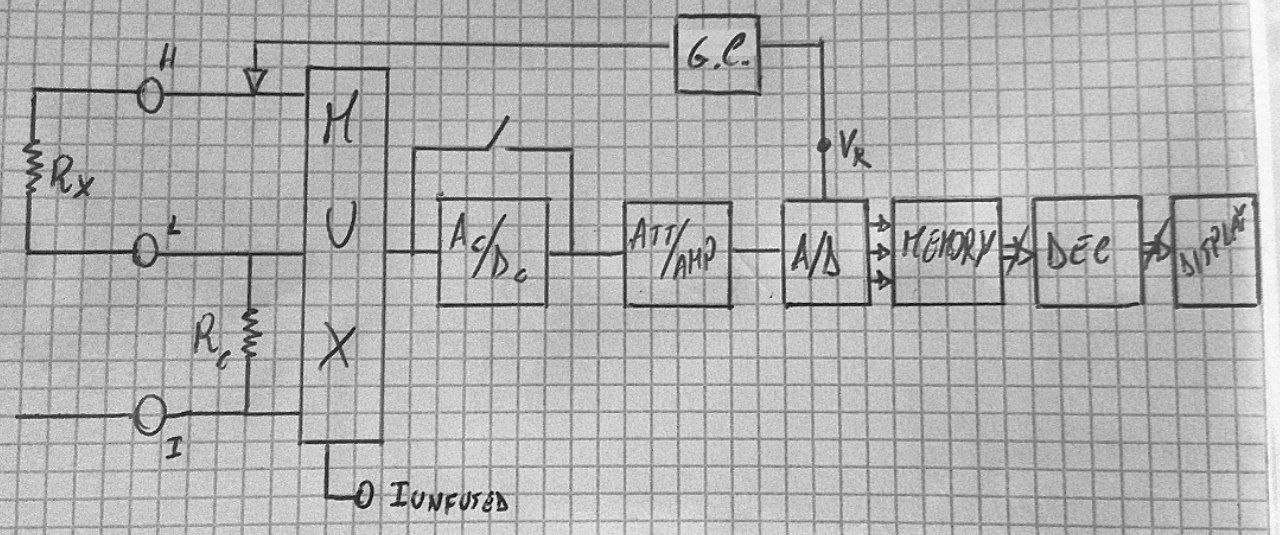
\includegraphics[width=\textwidth]{Images/figure1.jpg}
\end{center}
\section{Misurazione di tensioni continue e alternate}
Si può usare il \textbf{multimetro} come \textbf{voltmetro} , applicando la $V_x$ incognita tra i morsetti \textbf{H} e \textbf{L}.\\
I circuiti integrati forniscono in \textbf{uscita} una \textbf{tensione proporzionale} al \textbf{valore efficace} della tensione periodica presente al loro ingresso.
\section{Misurazione di correnti continue e alternate}
Per misurare \textbf{correnti} \textbf{continue} \textbf{alternate} si utilizzano i morsetti \textbf{I} e \textbf{L}, convertendo la \textbf{corrente} in una \textbf{tensione} facendo passare la \textbf{corrente} \textbf{incognita} in una \textbf{resistenza} \textbf{nota} $R_c$.
\section{Misurazione di resistenza a due e quattro fili}
Per eseguire misurazioni di resistenze a \textbf{due} \textbf{fili}, metto $R_x$ tra \textbf{H} e \textbf{L}.\\
Lo strumento impone la circolazione di una \textbf{corrente} sugli ordini di $mA$ nella \textbf{serie} costituita dalla \textbf{resistenza} $R_x$ e da $R_c$, connessa dai morsetti \textbf{(H-L)} e \textbf{(L-I)}.\\
Quindi si misurano $V_x \ e V_c \implies R_x = \frac{V_x}{V_c} \cdot R_c$